\chapter{Message Passing using Channels} 

We saw in the last chapter that we need some way to provide for
\emph{disciplined} interaction between threads, to avoid threads interfering
with one another.  In this book, we will see three basic ways to achieve this:
message passing, monitors and semaphores.  At a higher level of abstraction,
we will also see how to use concurrent datatypes.

We will start with message passing.  In my opinion, it is the most intuitive
approach: threads send messages to one another.  In addition, message passing
is necessary for distributed computing, and also works well with loosely
coupled systems.

A downside is that message passing tends to be slower than other approaches,
because there is an overhead in the sending and receiving of messages.
However, it is a good paradigm to start with, to get used to thinking about
concurrent programs.

The basic idea is that programs are composed of components, which might be
either threads (i.e.~sharing an address space) or processes (with distinct
address spaces, possibly on different computers).  These threads or processes
communicate only by sending and receiving messages over \emph{channels}.  In
this book, we will be dealing with threads; but the same techniques can be
used with processes.

%%%%%

\section{Defining and using channels}

Think of a channel as a wire.  Messages are sent at one end, and received at
the other end.

%% \item At one end there is an output port, at the other an input port.
%% %
%% \begin{center}
%% \begin{tikzpicture}
%% \draw (0,0) node[draw] (sender) {\scalashape chan!v};
%% \draw (4.5,0) node[draw] (receiver) {\scalashape chan?()};
%% \draw[->] (sender) -- 
%%   node[above,near start]{\small outport} 
%%   node[above,near end]{\small inport} (receiver);
%% \end{tikzpicture}
%% \end{center}

%% \item Values sent at the outport end (using |chan!v|) are received at the
%%   inport end (using |chan?()|), in the same order.

%% \item
%% Channels can be either synchronous or asynchronous; we will use a mix in this
%% course.
%% \end{itemize}
%% \end{slide}

%%%%%

In SCL, \SCALA{Chan[A]} is the type of channels that pass data of
type~\SCALA{A}.  This has  subtypes |SyncChan[A]|, of synchronous
channels, and |BuffChanT[A]|, of buffered (or asynchronous) channels.  We will
start by describing synchronous channels, and later describe buffered
channels. 

The command
\begin{scala}
  val chan = new SyncChan[A]
\end{scala}
defines |chan| to be a synchronous channel passing data of type~|A|.  Then the
command 
\begin{scala}
  chan!v
\end{scala}
sends the value \SCALA{v} on \SCALA{chan}.  The expression
\begin{scala}
  chan?()
\end{scala}
receives a value from~\SCALA{chan} and returns it.  The communication is
\emph{synchronous}: whichever part is executed first waits for the other; both
then proceed.  Thus the send and receive appear to take place at the same
time.  

%%%%%

For example, the following program prints the number 42 (in a round-about
way): 
\begin{scala}
  val chan = new SyncChan[Int]
  run(thread{ chan!42 } || thread{ println(chan?()) }) 
\end{scala}
%
This runs two threads: the first thread sends 42 on the channel; the second
thread receives a value on the channel, and prints it.

%%%%%

As another example, here's a function that produces a thread that repeatedly
inputs values from the channel \SCALA{in}, and outputs them on the
channel~\SCALA{out}:
%
\begin{scala}
  def copy[A](in: SyncChan[A], out: SyncChan[A]) = thread("copy"){
    while(true){ val x = in?(); out!x }
  }
\end{scala}
%
(The function is parameterised by the type~|A| of data passed on the channels,
and by the channels themselves.)
%
We could have written the body of \SCALA{copy} as simply:
\begin{scala}
  while(true) out!(in?()) 
\end{scala}
Note that in both forms, the communication on |in| can proceed even if no
thread is yet ready to receive on |out|.

%%%%%

A channel is simply an \emph{in-port} (something from which threads can
receive) and an \emph{out-port} (something on which threads can send). 
Note that the terminology ``in-port'' and ``out-port'' refer to the point of
view of \emph{threads}, not channels: a thread receives values in on an
in-port, and sends values out on an out-port; however, a value is put into a
channel on an out-port, and passed out on an in-port.

Figure~\ref{fig:channel-types} outlines the relevant types.  (The definition
of |Chan[A]| uses multiple inheritance: it inherits definitions from both
|InPort[A]| and |OutPort[A]|.)  The types \SCALA{InPort[A]} and
\SCALA{OutPort[A]} can be abbreviated as \SCALA{??[A]} and~\SCALA{!![A]},
respectively.

%%%%%%

\begin{figure}
\begin{scala}
package ox.scl.channel

trait InPort[A]{ def ?(): A; ... }
        
trait OutPort[A]{ def !(value: A): Unit; ... }
  
trait Chan[A] extends InPort[A] with OutPort[A]{ ... }

class SyncChan[A] extends Chan[A]{...} 
\end{scala}
\caption{Outline of the types of channels.}
\label{fig:channel-types}
\end{figure}

%%%%%

The earlier function \SCALA{copy} uses only the \SCALA{InPort} of \SCALA{in}
and the \SCALA{OutPort} of \SCALA{out}.  We therefore could have written the
definition as:
%
\begin{scala}
  def copy[A](in: ??[A], out: !![A]) = thread("copy"){ 
    while(true) out!(in?()) 
  }
\end{scala}
%
This signature makes clear what the thread does with each channel, and so
helps with documentation (the names of the channels also help).  In addition,
this style provides some  type safety: if, for example, the code tries to send
on~|in|, the compiler will give a type error. 

In-ports and out-ports can be shared: multiple threads can send at an
out-port; and multiple threads can receive at an in-port.  However,
each communication involves a \emph{single} sender and a \emph{single}
receiver: if multiple  threads try to send, the implementation of the channel
ensures that only one succeeds at a time; and likewise for receiving.  We will
not use any sharing of ports in this chapter, but we will in later chapters.

%%%%%%%%%%%%%%%%%%%%%%%%%%%%%%%%%%%%%%%%%%%%%%%%%%%%%%%%%%%%

\section{Example: printing multiples of four}

We now consider a slightly larger example, which is an instance of a paradigm
known as \emph{fine-grained concurrency}: the system is built from several
small components which are composed in parallel.  It is not a very
efficient--- or even sensible---way to create real programs.  We include such
examples here as they are a good way to get used to thinking about
concurrency---where multiple components work together---while keeping the
quantity of code small.  Also, such a program could be thought of as a model
of an electronic circuit, with components implemented in hardware and wired
together.

The program appears in Figure~\ref{fig:Mults4}. The overall effect is to print
the multiples of four.

The function |console(in)| defines a component that repeatedly reads a value
from \SCALA{in} and writes it to standard output.  The function
\SCALA{nats(out)} defines a component that sends the natural numbers, in
order, on \SCALA{out}.  The function \SCALA{alts(in, out)} defines a component
that copies alternate values read from \SCALA{in} to \SCALA{out}.

%%%%%

\begin{figure}
\begin{scala}
object Mults4{
  def console[A](in: ??[A]) = thread("console"){ while(true) println(in?()) }

  def nats(out: !![Int]) = thread("nats"){ 
    var n = 0; while(true){ out!n; n += 1 }
  }

  def alts[A](in: ??[A], out: !![A]) = thread("alts"){ 
    while(true){ out!(in?()); in?() } 
  }

  def system = {
    val x1, x2, x4 = new SyncChan[Int]
    nats(x1) || alts(x1, x2) || alts(x2, x4) || console(x4)
  }

  def main(args: Array[String]) = run(system)
}
\end{scala}
\caption{Printing multiples of four.}
\label{fig:Mults4}
\end{figure}

%%%%%

The definition of |system| creates appropriate channels and puts the
components together as illustrated below.
%
\begin{center}
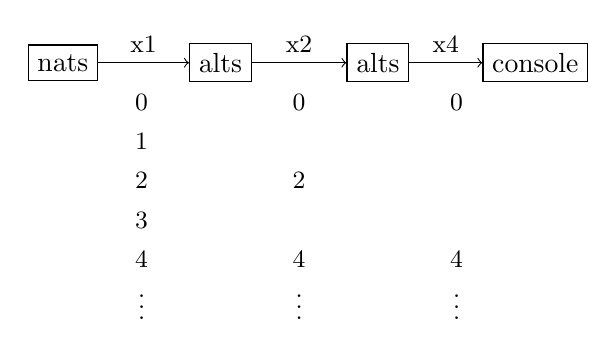
\begin{tikzpicture}
\draw (0,0) node[draw] (nats) {\scalashape nats};
\draw (nats)++(2,0) node[draw] (alts1) {\scalashape alts};
\draw[->] (nats) -- node[above]{\small\scalashape x1} (alts1);
\draw (alts1)++(2,0) node[draw] (alts2) {\scalashape alts};
\draw[->] (alts1) -- node[above]{\small\scalashape x2} (alts2);
\draw (alts2)++(2,0) node[draw] (console) {\scalashape console};
\draw[->] (alts2) -- node[above]{\small\scalashape x4} (console);
%
\draw (nats)++(1,-0.5) node {\small\scalashape 0};
\draw (nats)++(1,-1) node {\small\scalashape 1};
\draw (nats)++(1,-1.5) node {\small\scalashape 2};
\draw (nats)++(1,-2) node {\small\scalashape 3};
\draw (nats)++(1,-2.5) node {\small\scalashape 4};
\draw (nats)++(1,-3) node {\small\scalashape \vdots};
%
\draw (alts1)++(1,-0.5) node {\small\scalashape 0};
\draw (alts1)++(1,-1.5) node {\small\scalashape 2};
\draw (alts1)++(1,-2.5) node {\small\scalashape 4};
\draw (alts1)++(1,-3) node {\small\scalashape \vdots};
%
\draw (alts2)++(1,-0.5) node {\small\scalashape 0};
\draw (alts2)++(1,-2.5) node {\small\scalashape 4};
\draw (alts2)++(1,-3) node {\small\scalashape \vdots};
\end{tikzpicture}
\end{center}
%
The |nats| thread outputs the natural numbers on~|x1|.  The first instance of
|alts| receives these, and outputs every other value, i.e.~the even natural
numbers, on~|x2|.  The second instance of |alts| receives these, and outputs
every other value, i.e.~the multiples of four, on~|x4|.  |console| receives
these and prints them.  Thus the overall effect is to print the (non-negative)
multiples of~four.

\begin{instruction}
Make sure you understand how the components cooperate together.
\end{instruction}

%%%%%%%%%%%%%%%%%%%%%%%%%%%%%%%%%%%%%%%%%%%%%%%%%%%%%%%%%%%%

\section{Buffered channels}

In the previous examples, we used synchronous channels.  In effect, on each
channel, the send and receive of each value happen at the same time: the
sender and receiver \emph{synchronise} on the communication.
%
Using synchronous channels can make programs easier to understand: it helps us
to relate the states in different components.

By contrast, buffered channels normally allow a send to happen, even if there
is no thread ready to receive: the sender can return immediately, and the
channel stores the values until a receiver is ready to receive them.  In
particular, the channel ensures the messages are received in the same order in
which they are sent: the channel acts as a first-in first-out buffer.

There are various types of buffered channels in SCL, collected in the trait
|BuffChanT|: 
\begin{scala}
trait BuffChanT[A] extends Chan[A]
\end{scala}
%
One class of buffered channels is defined as follows. 
%
\begin{scala}
class UnboundedBuffChan[A] extends BuffChanT[A]
\end{scala}
%
As the name suggests, these channels have unbounded capacity. In principle,
they can store arbitrarily many messages, bounded only by the limits of
available memory.  Thus a sender can always insert its value into the buffer
and return immediately. 

In the multiples-of-four example, we could have defined the channels as 
%
\begin{scala}
  val x1, x2, x4 = new UnboundedBuffChan[Int]
\end{scala}
%
Making the channels buffered might help to overcome inconsistencies in the
speeds of threads.  For example, is one thread is suspended, its neighbours
will be able to continue.

A difficulty with using an unbounded buffer is that if the receiver is slower
than the sender, messages will accumulate in the buffer, using more and more
memory, possibly until the limits of available memory are reached.  This is
likely to be the case in the multiples-of-four pipeline, where the thread
printing results is likely to be slower than the other components. 

There are two types of bounded buffered channels within SCL.  Such channels
can hold a bounded number of values.  Once the bound is reached, the sender is
blocked until the receiver receives one of the earlier messages, and so makes
space in the channel.
%
The two types of bounded buffered channel are defined as:
%
\begin{scala}
class OnePlaceBuffChan[A] extends BuffChanT[A]
class BuffChan[A: scala.reflect.ClassTag](size: Int) extends BuffChanT[A]
\end{scala}
%
As the name suggests, a |OnePlaceBuffChan| is able to store just a single
piece of data.  However, |BuffChan|s are more flexible: each has a capacity
defined by its |size| parameter.

Choosing the correct capacity requires a combination of judgement and
guesswork.  Typically, neither the sender nor the receiver will try to
communicate at a constant rate, both because some data items will take longer
to process, and because either thread might be descheduled.  The buffering can
help to smooth out these irregularities.  Further, it is likely that they have
different long-term average rates of communication.  If the sender is, on
average, faster than the receiver, we would like enough buffering that the
receiver rarely has to wait for an item, i.e.~the buffer rarely becomes empty;
alternatively, if the receiver is, on average, faster than the sender, we
would like enough buffering that the sender rarely has to wait to deposit a
value, i.e.~the buffer rarely becomes full.  On the other hand, having too
much buffering uses additional memory.

\framebox{Experiments} 



%% However, the implementation of buffered channels imposes a bound on the number
%% of messages that can be buffered.  Suppose we did not have such a bound, and
%% imagine a scenario where the sender sent messages much faster than the
%% receiver could deal with them.  Then the buffered channel will hold more and
%% more messages, consuming more and more memory, possibly until all available
%% memory is used.  With a bounded buffered channel, once the bound is reached,
%% the sender is blocked until the receiver is ready to receive one of the
%% earlier messages. 

%%%%%

%% The class of buffered channels is defined as follows.
%% %
%% \begin{scala}
%% class BuffChan[A: scala.reflect.ClassTag](size: Int) extends Chan[A]
%% \end{scala}
%% %
%% Thus a declaration such as
%% \begin{scala}
%% val chan = new BuffChan[Int](size)
%% \end{scala}
%% defines a new buffered channel, passing |Int|s, able to hold at most |size|
%% messages.

The ``|[A: scala.reflect.ClassTag]|'' in the declaration of |BuffChan| needs
some explanation. Internally, a {\scalashape BuffChan} stores the buffered
messages in an array.  This means that the runtime implementation needs to
construct an |Array[A]|.  However, in order to do this, it needs to have what
is known as a |ClassTag| for~|A|, essentially information that tells the
runtime what |A| is.  If {\scalashape A} is a concrete type, e.g.~{\scalashape
  Int}, then compiler can provide the {\scalashape ClassTag}.  In such---very
common---cases, you don't need to provide the |ClassTag|: you can happily
ignore the issue.  However, if {\scalashape A} is declared as a polymorphic
type in some enclosing definition, it should be given the type bound
{\scalashape A: scala.reflect.ClassTag}, and the compiler will ensure a
{\scalashape ClassTag} is available.  For example, here's a version of the
earlier |copy| function that uses buffered channels: the type parameter |A| of
|copy| needs to be given the type bound.
%
\begin{scala}
  def copy[A: scala.Reflect.ClassTag](in: BuffChan[A], out: BuffChan[A]) = thread{
    while(true){ val x = in?(); out!x }
  }
\end{scala}
%
When |copy| is called with a concrete type for~|A|, the compiler will provide
the |ClassTag|.


 % Channels; multiples of 4; buffered channels
\section{Closing channels}

Often a component has to process a finite stream of data.  But how should the
end of the stream be signalled?  One way might be to send a special
``end-of-stream'' value.  But that assumes that we can find such a value,
namely a that won't be sent as a valid piece of data; and it will require
additional programming to send that value, and for the receiver to recognise
it and act appropriately.

Further, it can sometimes be useful for a receiver to indicate to the sender
that it is unable to accept any more data, which involves some form of
upstream signalling.

The way we deal with each of these scenarios is for the relevant thread to
close the channel. 
%
In SCL, if |in| is an |InPort| (e.g.~a channel), then |in.close()| closes it.
%
If |out| is an |OutPort| (e.g.~a channel), then |out.endOfStream()| closes it
for sending.  For a synchronous channel, this also closes it for receiving.
However, for a buffered channel, other threads can continue to receive until
the buffer becomes empty, at which point the channel becomes fully closed.

%%%%%

If a thread tries to send or receive on a channel that has been closed, it
throws a |Closed| exception, a subclass of the |Stopped| exception class.
(We will see another subclass of |Stopped| in Chapter~\ref{chap:alts}.)

Threads should normally catch such exceptions (see Scala
box~\ref{sb:try-catch}), and then do the right thing.  For a receiver, if the
closing represents the end of the data stream, then typically the thread
should terminate.  But if the thread is part of a larger network, such as a
pipeline, then typically the thread should first close channels to other
components, to signal to the next component in line that the stream is closed.

%% If such closing is possible, the thread should handle it appropriately,
%% normally closing its channels to pass the message on. 

\pagebreak[3]

Here's a new version of |alts| that does this.
%
\begin{mysamepage}
\begin{scala}
  def alts[A](in: ??[A], out: !![A]) = thread("alts"){ 
    try{ while(true){ out!(in?()); in?() } } 
    catch{ case _: Closed => in.close(); out.endOfStream() }
  }
\end{scala}
\end{mysamepage}
% 
If either sending or receiving fails, because the channel has been closed,
that operation throws a |Closed| exception, which is caught.  The overall
effect is that the thread exits the loop, and closes both channels.  
%
Note that closing a channel that is already closed has no effect.
Note also that there's no need to close a channel that is about to go out of
scope and be garbage collected. 

The above pattern is sufficiently common, that there's a construct to capture
it.
%
\begin{scala}
  repeat{ <command> }
\end{scala}
%
behaves much like
\begin{scala}
  while(true){ <command> }
\end{scala}
but catches |Stopped| exceptions, and so terminates cleanly if
\SCALA{<command>} throws such an exception.  Figure~\ref{fig:BoundedMults4}
illustrates this for the |nats|, |alts| and |console| functions.
%% For example:
%% %
%% \begin{scala}
%% def alts[A](in: ??[A], out: !![A]) = thread{ 
%%   repeat{ out!(in?()); in?() } 
%%   in.close(); out.endOfStream()
%% }
%% \end{scala}

%%%%%

It's sometimes useful to exit a loop for some reason other than a channel
being closed.  The construct
%
\begin{scala}
  repeat(guard){ <command> }
\end{scala}
%
behaves much like
\begin{scala}
  while(guard){ <command> }
\end{scala}
but terminates cleanly if \SCALA{<command>} throws a \SCALA{Stopped}
exception.

%%%%%%%%%%

Figure~\ref{fig:BoundedMults4} illustrates the technique of closing channels
via a version of the multiples-of-four example that prints up to some maximum
value~|max|, and then terminates cleanly.  This works by inserting a new
component into the pipeline, to close down the network once a value greater
than |max| is reached, as illustrated below.
%
\begin{center}
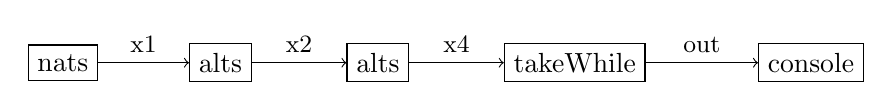
\begin{tikzpicture}
\draw (0,0) node[draw] (nats) {\scalashape nats};
\draw (nats)++(2,0) node[draw] (alts1) {\scalashape alts};
\draw[->] (nats) -- node[above]{\small\scalashape x1} (alts1);
\draw (alts1)++(2,0) node[draw] (alts2) {\scalashape alts};
\draw[->] (alts1) -- node[above]{\small\scalashape x2} (alts2);
\draw (alts2)++(2.5,0) node[draw] (takeWhile) {\scalashape takeWhile};
\draw[->] (alts2) -- node[above]{\small\scalashape x4} (takeWhile);
\draw (takeWhile)++(3,0) node[draw] (console) {\scalashape console};
\draw[->] (takeWhile) -- node[above]{\small\scalashape out} (console);
%
%% \draw (nats)++(1,-0.5) node {\small\scalashape 0};
%% \draw (nats)++(1,-1) node {\small\scalashape 1};
%% \draw (nats)++(1,-1.5) node {\small\scalashape 2};
%% \draw (nats)++(1,-2) node {\small\scalashape 3};
%% \draw (nats)++(1,-2.5) node {\small\scalashape 4};
%% \draw (nats)++(1,-3) node {\small\scalashape \vdots};
%% %
%% \draw (alts1)++(1,-0.5) node {\small\scalashape 0};
%% \draw (alts1)++(1,-1.5) node {\small\scalashape 2};
%% \draw (alts1)++(1,-2.5) node {\small\scalashape 4};
%% \draw (alts1)++(1,-3) node {\small\scalashape \vdots};
%% %
%% \draw (alts2)++(1,-0.5) node {\small\scalashape 0};
%% \draw (alts2)++(1,-2.5) node {\small\scalashape 4};
%% \draw (alts2)++(1,-3) node {\small\scalashape \vdots};
\end{tikzpicture}
\end{center}

%%%%%

\begin{figure}
\begin{scala}
object BoundedMults4{
  def nats(max: Int, out: !![Int]) = thread("nats"){ 
    var n = 0
    repeat{ out!n; n += 1 }
  }

  def alts[A](in: ??[A], out: !![A]) = thread("alts"){ 
    repeat{ out!(in?()); in?() }
    in.close(); out.endOfStream()
  }

  def console[A](in: ??[A]) = thread("console"){ repeat{ println(in?()) } }

  def takeWhile[A](p: A => Boolean, in: ??[A], out: !![A]) = thread("takeWhile"){
    var done = false
    repeat(!done){ val x = in?(); if(p(x)) out!x else done = true }
    in.close(); out.endOfStream()
  }

  def system(max: Int) = {
    val x1, x2, x4, out = new SyncChan[Int]
    nats(max, x1) || alts(x1, x2) || alts(x2, x4) || 
      takeWhile((x: Int) => (x <= max), x4, out) || console(out)
  }

  def main(args: Array[String]) = {
    val max = args(0).toInt; run(system(max))
  }
}
\end{scala}
\caption{Printing multiples of four, up to some maximum value.}
\label{fig:BoundedMults4}
\end{figure}

%%%%%

In fact, the new component is an instance of a more general pattern.  The
function |takeWhile(p, in, out)| copies data from~|in| to~|out| while all
values satisfy the predicate~|p| (the type \protect\SCALA{A => Boolean}
represents functions from~{\scalashape A} to~{\scalashape Boolean}; see Scala
box~\ref{sb:function-types}); it then closes the channels.

The other components are adapted to handle the closing of channels, using
|repeat|.  The |alts| components also close their channels, to indicate to
their neighbours that the system is terminating (in fact, the
``|out.endOfStream()|'' is unnecessary in this case because that part of the
network is closing in an upstream direction). 

The function |system| creates the channels and puts the components together in
parallel.  (In the first parameter of |takeWhile|, the notation \SCALA{(x:
  Int) => (x <= max)} represents the function that takes an |Int|
argument~|x|, and returns the result of the test |(x <= max)|; see Scala
box~\ref{sb:anon-function}.  In fact, the
parentheses around that test aren't necessary.)

\begin{instruction}
Make sure you understand how the termination signal is propagated through the
system. 
\end{instruction}
%\medskip

There are two other operations on channels related to closing. 
It is possible to test whether a channel~|c| is closed using the expression
%
\begin{scala}
  c.isClosed
\end{scala}
%
A closed channel~|c| can be reopened using the construct
\begin{scala}
  c.reopen()
\end{scala}
%
This has a precondition that the channel is indeed closed, and that no thread
is trying to send or receive on it.  This allows channels to be reused.

% \framebox{Cut above?}

%%%%%%%%%%%%%%%%%%%%%%%%%%%%%%%%%%%%%%%%%%%%%%%%%%%%%%%

\section{Example: producing the natural numbers}

We now consider another example of fine-grained concurrency, a circuit that
outputs the natural numbers.  The circuit is depicted below, and the code is
in Figure~\ref{fig:NatsCircuit}. 

\begin{center}
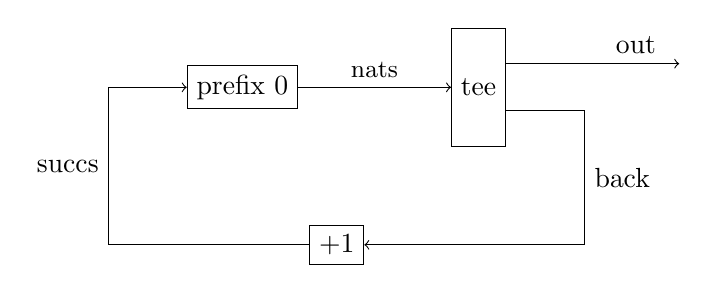
\begin{tikzpicture}
\draw(0,0) node[draw] (prefix) {\scalashape prefix 0};
% tee
\draw(prefix) ++(3,0) node[draw, minimum height = 15mm] (tee) {\scalashape tee};
\draw[->] (prefix) -- node[above]{\small\scalashape nats} (tee);
\draw[->] (tee.east)++(0,0.3) -- 
  node[above, near end]{\scalashape out} ++ (2.2,0);
% +1
\draw(prefix) ++ (1.2,-2) node[draw] (succ) {\scalashape +1};
\draw[->] (tee.east)++(0,-0.3) -- ++ (1.0,0) |-  
  node[right, near start]{\scalashape back} (succ);
\draw[->] (succ) -- ++(-2.9,0) |- 
  node[left, near start]{\scalashape succs} (prefix);
\end{tikzpicture}
\end{center}

%%%%%

\begin{figure}
\begin{scala}
object NatsCircuit{
  def console[A](in: ??[A]) = thread("console"){ repeat{ println(in?()) } }

  def prefix[A](x: A, in: ??[A], out: !![A]) = thread("prefix"){
    out!x; repeat{ out!in?() }
  }

  def tee[A](in: ??[A], out1: !![A], out2: !![A]) = thread("tee"){
    repeat{ val x = in?(); out1!x; out2!x }
  }

  def map[A,B](f: A => B, in: ??[A], out: !![B]) = thread("map"){
    repeat{ out!(f(in?())) }
  }

  def nats(out: !![Int]): ThreadGroup = {
    val nats, succs, back = new SyncChan[Int]
    prefix(0, succs, nats) || tee(nats, out, back) ||
      map(((x: Int) => x+1), back, succs)
  }

  def system: ThreadGroup = {
    val c = new SyncChan[Int]; nats(c) || console(c)
  }

  def main(args: Array[String]) = run(system)
}
\end{scala}
\caption{A concurrent circuit that outputs the natural numbers.}
\label{fig:NatsCircuit}
\end{figure}

The component labelled ``|prefix 0|'', produced using the function~|prefix|,
initially sends |0| on |nats|, and then copies values from |succs| to |nats|;
thus its output stream is its input stream prefixed by~|0|.  The component
labelled ``|tee|'', produced using the function~|tee|, copies values from
|nats| to both |out| and |back|.  The component labelled ``|+1|'' adds~|1| to
each value it receives on |back|, and outputs the result on |succs|; it is
produced by the function |map|, which generalises the particular functionality
we need, by applying the function~|f| to each value it receives.  Then |nats|
puts the components together, and |system| connects |nats| to a console
component.

Note that the circuit is cyclic.  Initially, |prefix 0| will produce~|0|; this
will be output and passed to |+1|.  The |+1| component will pass~|1| back to
|prefix 0|, via which it will be output and passed round the circuit.  And so
on.  In particular, it is important that |prefix 0| can send \emph{before} it
receives any value.  If every component started by trying to receive a value,
none would succeed, and the circuit would be deadlocked. 

\begin{instruction}
Make sure you understand how the circuit works, and how values propagate
round.
\end{instruction}

The above version of \SCALA{tee} outputs on its \SCALA{out1} channel before
its \SCALA{out2} channel.  That definition is fine in the context of the
circuit in question.  However, it could go wrong if used in the context of
some larger system that inputs on \SCALA{out2} before \SCALA{out1}.  For
example consider the following:
%
\begin{scala}
  val in, out1, out2 = new SyncChan[Int]
  def printer = thread("printer"){ println(out2?() + out1?()) } 
  run( tee(in, out1, out2) || printer)
\end{scala}
%
The printer thread will try to input on |out2| first (because |+| evaluates
its left-hand argument first).  But that means the system will get into a
deadlocked state, where the |tee| is blocked, trying to send on |out1|, and
the printer is blocked trying to receive on |out2|.  (Recall that in such
situations, typing \texttt{Ctrl}+$\backslash$ in the terminal produces a
thread dump, giving information about the running threads, which can be useful
for debugging.)

%% % %%%%%

%% Generic components should place as few assumptions as possible upon the
%% network in which they are placed. 
The following version of |tee| performs the outputs concurrently, which means
they can happen in either order.
%
\begin{mysamepage}
\begin{scala}
  def tee[A](in: ??[A], out1: !![A], out2: !![A]) = thread{
    repeat{ 
      val v = in?()
      run(thread{out1!v} || thread{out2!v}) 
    }
  }
\end{scala}
\end{mysamepage}
%
This version of |tee| will work fine in the context of the above system.  It
might be worth defining components in this style for generic components, or
when you don't know the order in which two communications will happen (and
this will be necessary in Exercise~\ref{ex:sorting}).  However, creating and
running two new threads is moderately expensive.  In specific settings, it
might be easier and more efficient to perform the outputs in a fixed order.
 % Closing channels; natural numbers
% Draw a comparator in the rows given by #1 and #2, with a horizontal
% displacement of #3
\def\comp#1#2#3{%
  \draw (#1)+(#3,0) node {$\bullet$};
  \draw (#2)+(#3,0) node (n2) {$\bullet$};
  \draw[thick] (#1)+(#3,0) -- (n2.center);
}


\framebox{Fine-grained concurrency}

%%%%%%%%%%

\section{Example: Quick Sort}

In this section we build a circuit of small threads.  The circuit inputs a
steam of |Int|s (with the end of stream signalled by the channel closing), and
then outputs a sorted version of that stream (and closes the channel to
indicate that).  The circuit is not the most practical way to sort numbers;
but it illustrates various ideas.

More precisely, we will write a  definition with the following signature
%
\begin{scala}
  def qSort(in: ??[Int], out: !![Int]): ThreadGroup = ...
\end{scala}
%
The function will produce a |ThreadGroup| that, when run, performs the
sorting.  The sorting will be based on the Quicksort algorithm.  That
algorithm is recursive, so the |qSort| function will also be recursive.

%%%%%

\framebox{Names for threads -- explain notation}

Suppose the input stream is empty.  Then |qSort| should just close its output
port to signal an empty output stream.  This can be achieved using the
following outline.
%
\begin{scala}
  def qSort(in: ??[Int], out: !![Int]): ThreadGroup = thread("QSort"){
    attempt{
      val pivot = in?()
      ...
    }{
      out.endOfStream // We've received no data, so just close
    }
  }
\end{scala}
%
The command |attempt{p}{q}| acts like~|p|, but if that throws a |Stopped|
exception, it executes~|q|.  Thus if the initial attempt to input on |in|
fails, the function performs |out.endOfStream|.

We now consider the resursive case.  Suppose the first input succeeds, giving
a value stored in |pivot|.  We then create two recursive |qSort| threads, that
will deal with values less than |pivot|, and at least pivot, respectively.  In
addition, a controller thread ties things together.  The controller
%
\begin{itemize}
\item Continues to input on |in|, passing values to the appropriate recursive
  |qSort| thread;

\item When |in| is closed, closes the channels to the recursive |qSort|s to
  signal the end of their input streams;

\item Receives the outputs from the recursive |qSorts|, and passes them along
  on |out|, along with |pivot|, in the appropriate order.
\end{itemize}
%
The following diagram illustrates how the controller communicates with the
recursive |qSort| processes.
%
\begin{center}
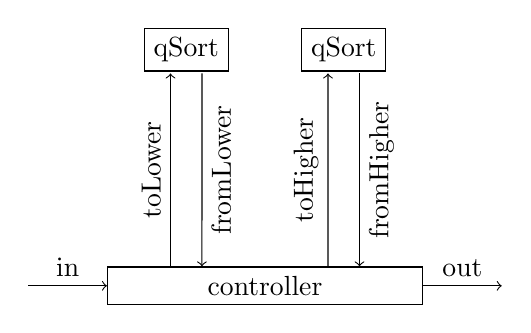
\begin{tikzpicture}
\draw (0,0) node[draw, minimum width=40mm] (controller) {\scalashape controller};
\draw[->] (controller.west) ++ (-1,0) -- 
   node[above]{\scalashape in} (controller.west);
\draw[<-] (controller.east)++(1,0)  -- 
   node[above]{\scalashape out} (controller.east);
%
\draw (controller) ++ (-1,3) node[draw] (rec1) {\scalashape qSort};
\draw (rec1.south)++(-0.2,0.1) node (rec1In) {};
\draw[->] (controller.north) ++ (-1.2,0.0) -- 
  node[above,sloped] {\scalashape toLower} (rec1In);
\draw (rec1.south)++(0.2,0.1) node (rec1Out) {};
\draw[<-] (controller.north) ++ (-0.801,0) -- 
  node[below,sloped] {\scalashape fromLower} (rec1Out);
%
\draw (controller) ++ (1,3) node[draw] (rec2) {\scalashape qSort};
\draw (rec2.south)++(-0.2,0.1) node (rec2In) {};
\draw[->] (controller.north) ++ (0.8,0.0) -- 
  node[above,sloped] {\scalashape toHigher} (rec2In);
\draw (rec2.south)++(0.2,0.1) node (rec2Out) {};
\draw[<-] (controller.north) ++ (1.2,0) -- 
  node[below,sloped] {\scalashape fromHigher} (rec2Out);
\end{tikzpicture}
\end{center}

%%%%%

The following definition implements this strategy.
%
\begin{scala}
  def qSort(in: ??[Int], out: !![Int]): ThreadGroup = thread("QSort"){
    attempt{
      val pivot = in?()
      val toHigher, toLower, fromHigher, fromLower = new SyncChan[Int]
      // Main controller thread.
      def controller = thread("Controller"){
        repeat{ val n = in?(); if(n < pivot) toLower!n else toHigher!n }
	toHigher.endOfStream; toLower.endOfStream
        repeat{ out!(fromLower?()) }; out!pivot; repeat{ out!(fromHigher?()) }
        out.endOfStream
      }      
      // Put the system together and run it.
      run(controller || qSort(toHigher, fromHigher) || qSort(toLower, fromLower))
    }{ out.endOfStream } // We've received no data, so just close
  }
\end{scala}

%%%%%  

Testing is an important part of programming.  Since concurrent programs tend
to be harder than sequential ones, testing is particularly important.

A general strategy for testing is to generate some random data, run the
parallel program on it, run a sequential program on it, and check that the two
give the same answer.  This can be repeated many times.  Of course, this
assumes that we have a correct sequential program for the same problem.  (In
fact, this strategy is also useful for testing sequential programs, where we
have a, typically simple, implementation that we are sure is correct, but we
want to test a more sophisticated program against it.)

%% Here's a strategy for testing:
%% %
%% \begin{enumerate}
%% \item Pass in values from an array~|xs| of random numbers;
%% \item Receive the outputs into an array~|ys|;
%% \item Check that |ys| is indeed a sorted version of~|xs|;
%% \item Repeat many times.
%% \end{enumerate}

The following code achieves this.
%
\begin{scala}
  import scala.util.Random
  val MaxSize = 100; val Max = 100
  def doTest{
    val size = Random.nextInt(MaxSize)
    val xs = Array.fill(size)(Random.nextInt(Max))
    val ys = new Array[Int](size)
    val in, out = new SyncChan[Int]
    def sender = thread("sender"){ for(x <- xs) in!x; in.endOfStream }
    def receiver = thread("receiver"){ var i = 0; repeat{ ys(i) = out?(); i += 1 } }
    run(sender || qSort(in, out) || receiver)
    assert(xs.sorted.sameElements(ys))
  }
\end{scala}
%
The |doTest| function performs a single test.  If uses an array |xs| of
size~|size|, where |size| is picked randomly in the range
$\interval{0}{\sm{MaxSize}}$; each element of |xs| is picked randomly in the
range $\interval{0}{\sm{Max}}$.  The |sender| thread sends the elements
of~|xs| to the |qSort| network on the |in| channel, then signals the end of
the stream.  The |receiver| thread receives the outputs from |qSort|, and
stores them in~|ys|.  The final line tests whether a sorted version of |xs|
(sorted using the |sorted| function from the Scala |Array| class) contains the
same elements as the outputs.

We can then run |doTest| many times:
%
\begin{scala}
  for(i <- 0 until 1000){ doTest; if(i%10 == 0) print(".") }
\end{scala}
%
This also intermittently prints a dot on the screen; this means that if the
system deadlocks for some reason, we will spot that it has got stuck!

%%%%%%%%%%%%%%%%%%%%%%%%%%%%%%%%%%%%%%%%%%%%%%%%%%%%%%%%%%%%

\heading{Practical 1: sorting networks}

The first practical asks you to implement various sorting algorithms using
fine-grained concurrency.  

Each sorting network will be built from \emph{comparators}: simple
two-element sorting components.  A comparator can be pictured as below: 
%
\begin{center}
\begin{tikzpicture}[scale = 0.8, >=angle 90,shorten >=1pt]
\node at (0,0.6) {comparator};
\draw (-2,-0.5) rectangle (2,1.5);
\node (x1) at (-5, -0.2) {$x_1$};
\node (x0) at (-5, 1.2) {$x_0$};
\draw[->] (x1) -- node[above]{ $in_1$} (-2,-0.2);
\draw[->] (x0) -- node[above]{ $in_0$} (-2,1.2);
\node (y1) at (6.5,-0.2) {$y_1 = max(x_0,x_1)$};
\node (y0) at (6.5,1.2) {$y_0 = min(x_0,x_1)$};
\draw[->] (2,-0.2) -- node[above]{ $out_1$} (y1);
\draw[->] (2,01.2) -- node[above]{ $out_0$} (y0);
\end{tikzpicture}
\end{center}
%
The comparator has two input channels, $in_0$ and $in_1$, and two output
channels, $out_0$ and $out_1$.  If it inputs $x_0$ and~$x_1$, it outputs their
minimum on~$out_0$ and their maximum on~$out_1$.

%%%%%

Below is a sorting network for four inputs using five comparators.
%
\begin{center}
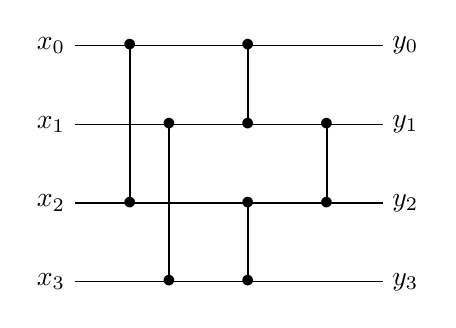
\begin{tikzpicture}
\draw (0,0) node (x0) {$x_0$};
\draw (0,-1) node (x1) {$x_1$};
\draw (0,-2) node (x2) {$x_2$};
\draw (0,-3) node (x3) {$x_3$};
\draw (4.5,0) node (y0) {$y_0$};
\draw (4.5,-1) node (y1) {$y_1$};
\draw (4.5,-2) node (y2) {$y_2$};
\draw (4.5,-3) node (y3) {$y_3$};
\draw (x0) -- (y0);
\draw (x1) -- (y1);
\draw (x2) -- (y2);
\draw (x3) -- (y3);
\comp{x0}{x2}{1}  \comp{x1}{x3}{1.5}
\comp{x0}{x1}{2.5}  \comp{x2}{x3}{2.5}
\comp{x1}{x2}{3.5}
\end{tikzpicture}
\end{center}
%
The first four comparators direct the smallest and largest values to the top
and bottom outputs; the final comparator sorts out the middle two values.

%%%%%%%%%%%%%%%%%%%%%%%%%%%%%%%%%%%%%%%%%%%%%%%%%%%%%%%%%%%%

\heading{Ordering of actions}

It is sometimes useful to consider an ordering over actions (memory reads and
writes, and sends and receives of messages) that talks about the order in
which those actions must happen.

We will write $a \preceq a'$, and say $a$ \emph{happens before}~$a'$, if (in a
particular execution of the program), $a'$ occur after, or simultaneously
with, $a$.

Note that if $a$ and $a'$ are a send and the corresponding receive over a
synchronous channel, then $a \preceq a'$ and $a' \preceq a$, so the relation
is not antisymmetric. 

%%%%%


We write $\equiv$ for the equivalence relation induced by~$\prec$:
\[
a \equiv a' \iff a \preceq a' \land a' \preceq a.
\]
This means that $a$ and~$a'$ happen at the same time, e.g.~the send and
receive on a synchronous channel.

We write $\prec$ for the strict version of~$\preceq$:
\[
a \prec a' \iff a \preceq a' \land a \not\equiv a.
\]
This means that $a$ happens strictly before~$a'$.

Formally, $\preceq$ is a preorder, i.e.~a transitive, reflexive order such
that:
%
\begin{itemize}
\item
If $a$ and $a'$ are actions of a single thread, and $a$ precedes $a'$, then $a
\prec a'$ (so $a \preceq a'$ but $a' \not\preceq a$);

\item
If $a$ is a send and $a'$ is the corresponding receive, then $a \preceq a'$
(regardless of whether the communication is over a synchronous or asynchronous
channel);  

\item
If $a$ is a receive and $a'$ is the corresponding send, and the communication
is over a synchronous channel, then $a \equiv a'$.
\end{itemize}

Note that some pairs of actions may be unrelated by~$\preceq$, so they can
happen in either order (necessarily in different threads).  In such cases, we
need to be sure that either order is acceptable --- i.e.~there is no race
condition. 

%%%%%%%%%%%%%%%%%%%%%%%%%%%%%%%%%%%%%%%%%%%%%%%%%%%%%%%%%%%%

\heading{Data-less channels}

It is sometimes useful to use a channel communication solely for
synchronisation between threads, rather than to pass any data.

This can be achieved in SCL using a channel that passes data of type
\SCALA{Unit}, the trivial type that contains a single value~\SCALA{()}.  

For example:
\begin{scala}
val c = new SyncChan[Unit]
run(thread{ print("Hello "); c!() } || thread{ c?(); println("world") })
\end{scala}

% This usage corresponds to simple events in CSP. 
We can reason using the happens-before relation.
\[
\sm{print("Hello")} \prec \sm{c!()} \equiv \sm{c?()} \prec \sm{println("world")}.
\]

The use of |!| and |?| could be reversed (but not with a buffered channel).

%%%%%%%%%%%%%%%%%%%%%%%%%%%%%%%%%%%%%%%%%%%%%%%%%%%%%%%%%%%%

\heading{Caching and compiler optimisations}

Recall that multiprocessor machines may cache variables, and that Java does
not guarantee that the caches will be kept coherent, so two concurrent
threads may operate independently on their own cached copies of the same
variable!  And further, the compiler is allowed to optimise the code to
something semantically equivalent as a sequential program.  The Java Memory
Model
%% \footnote{%
  %% \url{http://www.cs.umd.edu/~pugh/java/memoryModel/jsr-133-faq.html}.}
defines this more formally.

However, when two threads synchronise on a channel communication, any writes
made by one thread before the synchronisation are guaranteed to be visible to
the other thread after the synchronisation.  
%  reads or write a channel, the updates in its cache are
% flushed to main memory, and cached values re-read from main
% memory. 
Further compiler optimisations may not reorder events to break this.


%%%%%

For example, in the code
\begin{scala}
val c = new SyncChan[Unit]
var x = -1
def p = thread{ x = 42; c!() }
def q = thread{ c?(); <use x> }
run(p || q)
\end{scala}
%
\SCALA{q} is guaranteed to use the value |42| for \SCALA{x} written
by~\SCALA{p} because:
%
\begin{itemize}
\item 
\SCALA{p} finishes writing before the synchronisation;

\item
The synchronisation ensures the caches are correctly updated;

\item
The compiler is not allowed to perform optimisations that reorder the accesses
to~\SCALA{x} with those to~\SCALA{c}.
\end{itemize}

%%%%%

\heading{Rule for disciplined interaction}

Earlier we said that parallel threads should use \emph{disjoint} sets of
variables.  We can weaken this slightly, to allow threads to share
variables, as long as they do so in a disciplined way. 

If two threads both access a variable (other than both reading it) then
there should be a (direct or indirect) synchronisation between the threads
after the first finishes accessing the variable, and before the second starts
accessing it.  In particular, this avoids race conditions: the second thread
``knows'' the first has finished with the variable.  The Java Memory Model
avoids problems with caching and compiler optimisations.

You should state clearly which threads may read or write variables in
different states, and this should be done to avoid race conditions.

%%%%%

\heading{Objects and message passing}

Reference objects can be passed across channels in the same way as simpler
types.  (The channel passes the reference rather than the object itself.)

However, this needs to be done with care: if two threads share an object,
there is the danger of race conditions, just as with standard shared
variables. 
 
Note, in particular, that reference objects are passed by reference rather
than by value: sometimes it is necessary to copy objects, rather than simply
passing them, to avoid unintended sharing.

Consider \SCALA{p(in, mid) || q(mid)} where
%
\begin{scala}
def p(in: ??[String], mid: ![Person]) = thread{
  val pers = new Person()
  while(true){ val n = in?(); pers.name = n; mid!pers }
}

def q(mid: ??[Person]) = thread{
  while(true){ val pers = mid?(); println(pers.name) }
} 
\end{scala}
%
What is wrong with this?

%%%%%

\heading{Object-oriented versus thread-oriented programming}

Objects and threads can both be thought of as forms of
\emph{modularisation}. 

In object-oriented systems, many objects can exist simultaneously, each with
its own state.  Normally, a single one is active at a time.  They communicate
by procedure calls, which pass data and control.

In thread-oriented systems, many threads can exist simultaneously, each
with its own state, and (often) all active at the same time.  They communicate
by sending and receiving messages, which pass data.

Sometimes an individual thread will use multiple objects.  Sometimes objects
encapsulate threads.

%%%%%

\heading{Other approaches}

\begin{itemize}
\item Concurrent Scala Objects (CSO) is an API developed by Bernard Sufrin.
  SCL is heavily based on CSO.

\item Go\footnote{\url{https://golang.org/}} is a programming language created
by Google, using CSP-style channels.  It is probably the most
mainstream such language.

\item
{\sf occam} is a programming language based on CSP, and developed by INMOS in
the early 1980s.

\item Erlang uses similar ideas, in a functional setting.

\item JCSP\footnote{\url{http://www.cs.kent.ac.uk/projects/ofa/jcsp/}} is an
implementation of CSP for Java.

% \item Eclectic
% CSP\footnote{\url{http://users.comlab.ox.ac.uk/bernard.sufrin/ECSP/ecsp.pdf}}
% is an experimental language based on CSP, and a precursor of CSO.

%% \item Communicating Haskell
%% Processes\footnote{\url{http://www.cs.kent.ac.uk/projects/ofa/chp/}} is a
%% Haskell library to support CSP-style communication.

\item Rust supports concurrency in a number of styles, including message
  passing\footnote{%
    \url{https://doc.rust-lang.org/book/ch16-02-message-passing.html}}. 

% \item
% There are various experimental languages based on Python with CSP-style
% communication. 
\end{itemize}


%%%%%
 % merge sort; order of actions

%%%%%%%%%%%%%%%%%%%%%%%%%%%%%%%%%%%%%%%%%%%%%%%%%%%%%%%% %%%%%

\section{Summary}

In this chapter we have seen the basics of message passing concurrency.  The
idea is straightforward: threads can send messages to one another.

We have arranged that threads have no shared variables.  This means that we
avoid any memory races, of the form that we saw in Chapter~\ref{chap:intro}.
In later chapters, we will relax this condition, and allow some shared
variables.  However, we will still need to ensure disciplined access to those
variables, and message passing will be one technique that we can use to
coordinate the threads.  

We have seen how to use message passing using the SCL library.  Threads
communicate via \emph{channels}, which comprise an \emph{in-port} and an
\emph{out-port}.  Threads can send messages at an out-port, which are received
at the corresponding in-port.  Channels can be either \emph{synchronous} or
\emph{asynchronous} (buffered).  A port can be shared between several threads.
Channels can be closed, for example to indicate the end of a stream of data;
and this can be used to signal the termination of a concurrent network.  

We have seen a number of examples illustrating message passing.  These have
mostly used fine-grained concurrency, where systems are built from very small
components.  The exercises at the end of this chapter include similar
examples.  Our aim in these examples has been to illustrate how concurrent
components can cooperate together.

We have also seen a technique for reasoning about concurrent programs, using
the ``happens-before'' relation ($\preceq$).

%%%%% 

\paragraph{Object-oriented versus thread-oriented programming}

An important part of programming is \emph{modularisation}: splitting a large
program up into manageable chunks.  The most common modularisation technique
is object orientation, where objects encapsulate some data and operations on
that data.  However, concurrency is also a form of modularisation, where each
thread holds some data, and communicates the results of operations on that
data with other threads.

In object-oriented systems, many objects can exist simultaneously, each with
its own state.  Normally, a single one is active at a time.  They communicate
by procedure calls, which pass data and control.

In message-passing concurrent systems, many threads can exist simultaneously,
each with its own state.  Often, all are active at the same time.  They
communicate by sending and receiving messages, which pass data.

The two techniques are complementary.  In later chapters, we will sometimes
encapsulate a thread inside an object.  And sometimes an individual thread
will use multiple objects, either as private objects or shared with other
threads. 

%%%%% 

\paragraph{Other approaches}

In this book, we use Scala together with the Scala Concurrency Library (SCL).
However, message-passing concurrency can also be used in a number of other
languages or with different concurrency primitives.

Message-passing concurrency started with the programming language {\sf occam}.
It was developed by INMOS in the early 1980s, targeting their transputer
microprocessors.

Concurrent Scala Objects (CSO) is a library of concurrency primitives, mostly
message-passing, developed by Bernard Sufrin.  SCL is heavily based on CSO,
and inherits much of the same syntax.  

Go\footnote{\url{https://golang.org/}} is a programming language created
by Google that uses message passing.  It is probably the most
mainstream such language.


Rust supports concurrency in a number of styles, including message
  passing\footnote{%
    \url{https://doc.rust-lang.org/book/ch16-02-message-passing.html}}. 
Erlang uses similar ideas, in a functional setting.

Message-passing libraries are available for a number of other languages.  For
example, JCSP\footnote{\url{http://www.cs.kent.ac.uk/projects/ofa/jcsp/}} is
an implementation  for Java.

% \item Eclectic
% CSP\footnote{\url{http://users.comlab.ox.ac.uk/bernard.sufrin/ECSP/ecsp.pdf}}
% is an experimental language based on CSP, and a precursor of CSO.

%% \item Communicating Haskell
%% Processes\footnote{\url{http://www.cs.kent.ac.uk/projects/ofa/chp/}} is a
%% Haskell library to support CSP-style communication.


% \item
% There are various experimental languages based on Python with CSP-style
% communication. 



%%%%%%%%%%%%%%%%%%%%%%%%%%%%%%%%%%%%%%%%%%%%%%%%%%%%%%%

\exercises

\begin{questionS}
Implement a variant of the |NatsCircuit| program from
Figure~\ref{fig:NatsCircuit} that receives an input~|max| (say from the command
line) and produces the natural numbers up to~|max| (inclusive), and then
terminates cleanly.
\end{questionS}

\begin{answerS}
We use the |takeWhile| function from Figure~\ref{fig:BoundedMults4}, and
insert a suitable component between the |prefix 0| and |tee| components.  
\begin{scala}
  def nats(max: Int, out: !![Int]): ThreadGroup = {
    val nats, nats1, succs, back = new SyncChan[Int]
    prefix(0, succs, nats) || takeWhile((x: Int) => x <= max, nats, nats1) ||
      tee(nats1, out, back) || map((x: Int) => x+1, back, succs)
  }
\end{scala}
We also adapt the |prefix|, |tee| and |map| functions so that each closes its
output channel when its |repeat| loop terminates (strictly speaking, this
isn't necessary for |prefix|).  Thus, when the |takeWhile| component receives
a value greater than |max|, the termination signal gets passed round the
circuit.
\end{answerS}

%% \begin{scala}
%% /** A fine-grained concurrent network that prints the natural numbers up to a
%%   * limit provided on the command line. */
%% object BoundedNatsCircuit{
%%   /** Repeatedly input on `in`, printing the values received. */
%%   def console[A](in: ??[A]) = thread{ repeat{ println(in?()) } }

%%   /** Copy from `in` to `out`, prefixing with `x`. */
%%   def prefix[A](x: A, in: ??[A], out: !![A]) = thread{
%%     out!x; repeat{ out!in?() }; out.endOfStream()
%%   }

%%   /** Copy values from `in` to both `out1` and `out2`. */
%%   def tee[A](in: ??[A], out1: !![A], out2: !![A]) = thread{
%%     repeat{ val x = in?(); out1!x; out2!x }
%%     out1.endOfStream(); out2.endOfStream()
%%   }

%%   /** Apply `f` to all values received on `in`, and output on `out`. */
%%   def map[A,B](f: A => B, in: ??[A], out: !![B]) = thread{
%%     repeat{ out!(f(in?())) }; out.endOfStream()
%%   }

%%   def takeWhile[A](p: A => Boolean, in: ??[A], out: !![A]) = thread{
%%     var done = false
%%     repeat(!done){ 
%%       val x = in?(); if(p(x)) out!x else done = true
%%     }
%%     out.endOfStream()
%%   }

%%   /** The network. */
%%   def nats(max: Int, out: !![Int]): ThreadGroup = {
%%     val nats, nats1, succs, back = new SyncChan[Int]
%%     prefix(0, succs, nats) || takeWhile((x: Int) => x <= max, nats, nats1) ||
%%       tee(nats1, out, back) || map((x: Int) => x+1, back, succs)
%%   }

%%   def system(max: Int) = {
%%     val c = new SyncChan[Int]; nats(max, c) || console(c)
%%   }

%%   def main(args: Array[String]) = {
%%     val max = args(0).toInt; run(system(max))
%%   }
%% }
 % bounded version of NatsCircuit

\begin{question}
\emph{Hamming numbers} are numbers whose only prime factors are $2$, $3$,
and~$5$.  Hence the first few Hamming numbers are:
\[ \mstyle
1, 2, 3, 4, 5, 6, 8, 9, 10, 12, 15, 16.
\]
Thus each Hamming number is either~$1$, or an earlier Hamming number
multiplied by~$2$, $3$, or~$5$.

The Hamming numbers can be produced by a circuit as depicted below.
%
\begin{center}
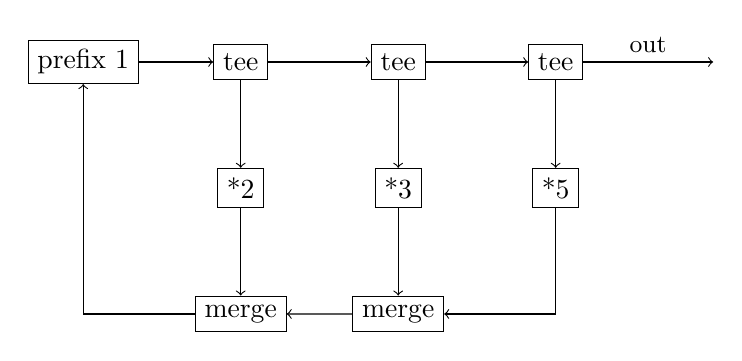
\begin{tikzpicture}[yscale = 0.8]
\draw (0,0) node[draw] (prefix) {\scalashape prefix 1};
% (*2) branch
\draw (prefix) ++ (2,0) node[draw] (tee2) {\scalashape tee};
\draw[->] (prefix) -- (tee2);
\draw (tee2) ++ (0,-2) node[draw] (mult2) {\scalashape *2};
\draw[->] (tee2) -- (mult2);
% (*3) branch
\draw (tee2) ++ (2,0) node[draw] (tee3) {\scalashape tee};
\draw[->] (tee2) -- (tee3);
\draw (tee3) ++ (0,-2) node[draw] (mult3) {\scalashape *3};
\draw[->] (tee3) -- (mult3);
% (*5) and out branch
\draw (tee3) ++ (2,0) node[draw] (tee4) {\scalashape tee};
\draw[->] (tee3) -- (tee4);
\draw (tee4) ++ (0,-2) node[draw] (mult5) {\scalashape *5};
\draw[->] (tee4) -- (mult5);
\draw[->] (tee4) -- node[above] {\small\scalashape out} ++ (2,0);
% merge of (*3) and (*5)
\draw (mult3) ++ (0,-2) node[draw] (merge1) {\scalashape merge};
\draw[->] (mult5) |- (merge1);
\draw[->] (mult3) -- (merge1);
% merge with (*2)
\draw (mult2) ++ (0,-2) node[draw] (merge2) {\scalashape merge};
\draw[->] (merge1) -- (merge2);
\draw[->] (mult2) -- (merge2);
% close loop
\draw[->] (merge2) -| (prefix);
\end{tikzpicture}
\end{center}
%
The |prefix 1| and |tee| components are as in Figure~\ref{fig:NatsCircuit}.
The |*2|, |*3|, and~|*5| components multiply their inputs by~$2$, $3$ and~$5$,
respectively.  The |merge| components receives two strictly increasing streams
and merges them together into a single strictly increasing stream; note that
this involves removing duplicate values, so this is slightly different from
the |merge| component we used in Section~\ref{sec:mergesort}.

Thus the |prefix 1| component sets things going; the |*2|, |*3|, and |*5|
components produce appropriate multiples; and the |merge| components merge the
streams together.

\begin{enumerate}
\item Implement the circuit using synchronous channels.  You will find that
  the system deadlocks.  Why is this?

\item Adapt the network to use buffered channels, where appropriate.  Is finite
  buffering enough?

\item Adapt the network so that it produces outputs only up to some given
  maximum value, and then terminates cleanly.
\end{enumerate}
\end{question}

%%%%%%%%%%%%%%%%%%%%%%%%%%%%%%%%%%%%%%%%%%%%%%%%%%%%%%%

\begin{answerI}
The |*2|, |*3|, and~|*5| components are simply instances of~|map|.

The |merge| function can be written as follows.  This meaintains the invariant
that  |l| is the last value read from |left|, and |r| is the last value read
from |right|.  In this example, closing of channels is just used to signal
termination, so we do not need to worry about outputting remaining inputs.
%
\begin{scala}
  def merge(left: ??[Int], right: ??[Int], out: !![Int]) = thread("Merge"){
    var l = left?(); var r = right?()
    repeat{
      if(l < r){ out!l; l = left?() }
      else if(l == r){ out!l; l = left?(); r = right?() }
      else{ out!r; r = right?() }
    }
    left.close(); right.close(); out.endOfStream()
  }
\end{scala}

The following function produces the system (including the latter part of the
question).
%
\begin{scala}
def system(out: !![Int], max: Int) = {
  val h0, h1, h2 = new SyncChan[Int]     // Inputs into £tee£ components.
  val i2, i3, i5 = new SyncChan[Int]     // Inputs into £*2£, £*3£, £*5£.
  val t2, t3, t5 = new UnboundedBuffChan[Int] // Outputs from £*2£, £*3£, £*5£.
  val m1, m2, m3 = new SyncChan[Int]    // Outputs from £merge£s and £takeWhile£.
  prefix(1, m3, h0) || tee(h0, i2, h1) || tee(h1, i3, h2) || tee(h2, i5, out) ||
  map((x:Int) => 2*x, i2, t2) || map((x:Int) => 3*x, i3, t3) || 
  map((x:Int) => 5*x, i5, t5) ||  
  merge(t2, t3, m1) || merge(t5, m1, m2) || 
  takeWhile((x: Int) => x <= max, m2, m3)
}
\end{scala}

The system without buffering deadlocks, basically because there are too many
intermediate values passing round the system for the various components to
hold.  In a bit more details, suppose the |prefix| component has just passed
a value~$n$.  Then the |*2| component will have output most of the Hamming
numbers less than $2n$; I say ``most'', because there might be a couple of
Hamming numbers either still in the |*2| component or the previous |tee|
component.  But that means that most of the Hamming numbers between $n$
and~$2n$ have to be stored somewhere in the subcircuit between the |*2| and
|prefix| components---and there simply isn't enough capacity for all of them. 
 
I use a buffered channel for the output from the |*2| component to store
them.  In fact, the number of Hamming numbers between~$n$ and~$2n$ tends to
infinity as $n$ tends to infinity, so we need an unbounded buffer.  The same
is true for the |*3| and |*5| components. 

To achieve termination, I inserted a |takeWhile| component just before the
|prefix| component---but it could have been inserted pretty much anywhere.
Also, each component is adapted to close its output channels when its main
loop terminates, and also arrange for the |takeWhile| and |merge| components
to close their input channels; the latter is necessary, or else we can get
into a situation where one of those components is trying to send to another,
but the latter has terminated, so the network is deadlocked.  There's no harm
in \emph{every} component closing its input channels.
\end{answerI}
 % Hamming numbers

\input{Exercises/pipesort} % sorting using a pipeline.

\begin{questionS}
Write a function
\begin{scala}
  def qSort(in: ??[Int], out: !![Int]): ThreadGroup
\end{scala}
that receives a stream of data on |in|, and outputs a sorted version on~|out|.
The sorting should be done using the Quicksort algorithm.  In the case that
the input stream contains at least one value, starting with a value~|pivot|,
use two recursive calls to |qSort| to sort the values that are less
than~|pivot|, and the other values that are greater than or equal to~|pivot|,
respectively.

Test your code. 
\end{questionS}

%%%%%%%%%%%%%%%%%%%%%%%%%%%%%%%%%%%%%%%%%%%%%%%%%%%%%%%

\begin{answerS}
My code is below.  I use an |attempt| structure to deal with the case that the
input stream is empty.  Otherwise, I build the system below, with two
recursive calls to |qSort|, and a controller tying them together.
%
\begin{center}
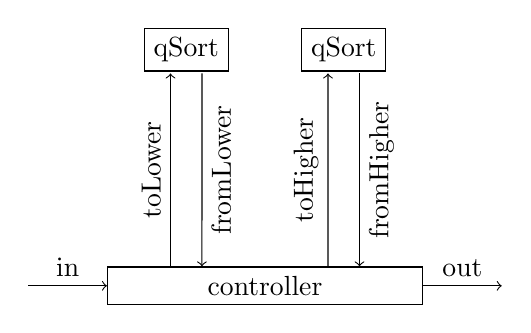
\begin{tikzpicture}
\draw (0,0) node[draw, minimum width=40mm] (controller) {\scalashape controller};
\draw[->] (controller.west) ++ (-1,0) -- 
   node[above]{\scalashape in} (controller.west);
\draw[<-] (controller.east)++(1,0)  -- 
   node[above]{\scalashape out} (controller.east);
%
\draw (controller) ++ (-1,3) node[draw] (rec1) {\scalashape qSort};
\draw (rec1.south)++(-0.2,0.1) node (rec1In) {};
\draw[->] (controller.north) ++ (-1.2,0.0) -- 
  node[above,sloped] {\scalashape toLower} (rec1In);
\draw (rec1.south)++(0.2,0.1) node (rec1Out) {};
\draw[<-] (controller.north) ++ (-0.801,0) -- 
  node[below,sloped] {\scalashape fromLower} (rec1Out);
%
\draw (controller) ++ (1,3) node[draw] (rec2) {\scalashape qSort};
\draw (rec2.south)++(-0.2,0.1) node (rec2In) {};
\draw[->] (controller.north) ++ (0.8,0.0) -- 
  node[above,sloped] {\scalashape toHigher} (rec2In);
\draw (rec2.south)++(0.2,0.1) node (rec2Out) {};
\draw[<-] (controller.north) ++ (1.2,0) -- 
  node[below,sloped] {\scalashape fromHigher} (rec2Out);
\end{tikzpicture}
\end{center}
%
The controller distributes input values to the two sub-sorters, depending on
how it compares with~|pivot|.  When the input stream is closed, it closes its
channels to the sub-sorters, to indicate that their input streams are
finished.  It then takes outputs from the two sub-sorters, and passes them
out, together with |pivot|, in the right order.
%
\begin{scala}
  def qSort(in: ??[Int], out: !![Int]): ThreadGroup = thread("QSort"){
    attempt{
      val pivot = in?()
      val toHigher, toLower, fromHigher, fromLower = new SyncChan[Int]
      // Controller thread.
      def controller = thread("Controller"){
	// Split data received on £in£ between £higher£ and £lower£, depending on
	// whether it is £$\ge \sm{pivot}$£ or £$< \sm{pivot}$£, respectively.
	repeat{ val x = in?(); if(x < pivot) toLower!x else toHigher!x }
	// We've received the final input, so close the channels to the
	// sub-sorters.
	toHigher.endOfStream(); toLower.endOfStream()
	// Now output the results.
	repeat{ out!(fromLower?()) }; out!pivot; repeat{ out!(fromHigher?()) }
	out.endOfStream()
      }      
      // Put the system together, and run it.
      run(controller || qSort(toHigher, fromHigher) || qSort(toLower, fromLower))
    }{ out.endOfStream() } // We've received no data, so just close.
  }
\end{scala}
\end{answerS}


% Draw a comparator in the rows given by #1 and #2, with a horizontal
% displacement of #3
\def\comp#1#2#3{%
  \draw (#1)+(#3,0) node {$\bullet$};
  \draw (#2)+(#3,0) node (n2) {$\bullet$};
  \draw[thick] (#1)+(#3,0) -- (n2.center);
}


\begin{question}
This question builds some networks to sort a list of numbers.  The networks
are not very sensible as software sorting networks; however, they could be
implemented efficiently in hardware. 
%%  The main aims of the practical are to help you get used to thinking about
%% concurrent systems, and to gain familiarity with the SCL library.

Each sorting network will be built from \emph{comparators}: simple
two-element sorting components.  A comparator can be pictured as below: 
%
\begin{center}
\begin{tikzpicture}[scale = 0.6, >=angle 90,shorten >=1pt]
\node at (0,0.6) {comparator};
\draw (-2,-0.5) rectangle (2,1.5);
\node (x1) at (-5, -0.2) {$x_1$};
\node (x0) at (-5, 1.2) {$x_0$};
\draw[->] (x1) -- node[above]{\scalashape\small in1} (-2,-0.2);
\draw[->] (x0) -- node[above]{\scalashape\small in0} (-2,1.2);
\node (y1) at (7.2,-0.2) {$y_1 = max(x_0,x_1)$};
\node (y0) at (7.2,1.2) {$y_0 = min(x_0,x_1)$};
\draw[->] (2,-0.2) -- node[above]{\scalashape\small out1} (y1);
\draw[->] (2,01.2) -- node[above]{\scalashape\small out0} (y0);
\end{tikzpicture}
\end{center}
%
The comparator has two input channels, |in0| and |in1|, and two output
channels, |out0| and |out1|.  If it inputs $x_0$ and~$x_1$, it outputs their
minimum on~|out0| and their maximum on~|out1|.

\begin{qpart} 
Implement a comparator with the following signature:
%
\begin{scala}
  /** A single comparator, inputting on £in0£ and £in1£, and outputting on £out0£
    * (smaller value) and £out1£ (larger value). */
  def comparator(in0: ??[Int], in1: ??[Int], out0: !![Int], out1: !![Int]): ThreadGroup
\end{scala}
%
the process should be willing to perform the inputs in either order, and
perform the outputs in either order.  The process should repeat this behaviour
until one of its channels is closed, at which point it should terminate.
\end{qpart}

%%%%%

Below is a sorting circuit for four inputs using five comparators.
%
\begin{center}
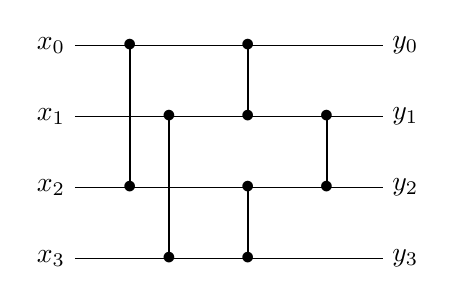
\begin{tikzpicture}[yscale = 0.9]
\draw (0,0) node (x0) {$x_0$};
\draw (0,-1) node (x1) {$x_1$};
\draw (0,-2) node (x2) {$x_2$};
\draw (0,-3) node (x3) {$x_3$};
\draw (4.5,0) node (y0) {$y_0$};
\draw (4.5,-1) node (y1) {$y_1$};
\draw (4.5,-2) node (y2) {$y_2$};
\draw (4.5,-3) node (y3) {$y_3$};
\draw (x0) -- (y0);
\draw (x1) -- (y1);
\draw (x2) -- (y2);
\draw (x3) -- (y3);
\comp{x0}{x2}{1}  \comp{x1}{x3}{1.5}
\comp{x0}{x1}{2.5}  \comp{x2}{x3}{2.5}
\comp{x1}{x2}{3.5}
\end{tikzpicture}
\end{center}
%
The first four comparators direct the smallest and largest values to the top
and bottom outputs; the final comparator sorts out the middle two values.
Note that the first two comparators can run concurrently, as can the second
pair: the longest path involves  three comparators.

\begin{qpart}
\label{Q:sort4}
Implement this sorting circuit, using the following
signature.%% \footnote{The class {\scalashape List} represents lists.  If
  %% you haven't used this class before, you might want to look at the
  %% API documentation, or a relevant on-line tutorial.}
%  
\begin{scala}
  /** A sorting network for four values. */
  def sort4(ins: List[??[Int]], outs: List[!![Int]]): ThreadGroup = {
    require(ins.length == 4 && outs.length == 4)
    ...
  }
\end{scala}
%
Test your implementation using the following idea: pick four random |Ints|,
and send them in on the input channels; receive the outputs and check that
they are a sorted version of the inputs; repeat many times.
\end{qpart}

%%%%%

We will  implement a sorting network based on the idea of insertion sort.
%
First, we need a circuit to insert a value into a sorted list of
$n \ge 1$ values, with the following signature.
%
\begin{mysamepage}
\begin{scala}
  /** Insert a value input on £in£ into a sorted sequence input on £ins£. 
    * Pre: £ins.length£ = £n£ and £outs.length = n+1£, for some £$\sm n \ge 1$£.
    * If the values £$xs$£ input on £ins£ are sorted, and £$x$£ is input on £in£, then a
    * sorted permutation of £$x::xs$£ is output on £ys£. */
  def insert(ins: List[??[Int]], in: ??[Int], outs: List[!![Int]]): ThreadGroup = {
    val n = ins.length; require(n >= 1 && outs.length == n+1)
    ...
  }
\end{scala}
\end{mysamepage}
%
Consider the circuit below to implement |insert|, for $\sm n \ge 2$.  The box
labelled ``$\sm{insert}_{\ss n-1}$'' is (recursively) a circuit to insert the
output of the comparator into the sorted list of values received on
$\sm{ins(1)}, \ldots, \sm{ins(n-1)}$. %  of length~$\sm n-1$.
%
%
\begin{center}
\def\width{6.5} % x coord for output labels
\def\recX{2} % X coord for start of recursive insert
\def\recWidth{3} % width of recursive insert
\def\recEnd{\recX+\recWidth} % X coord of right edge of recursive insert
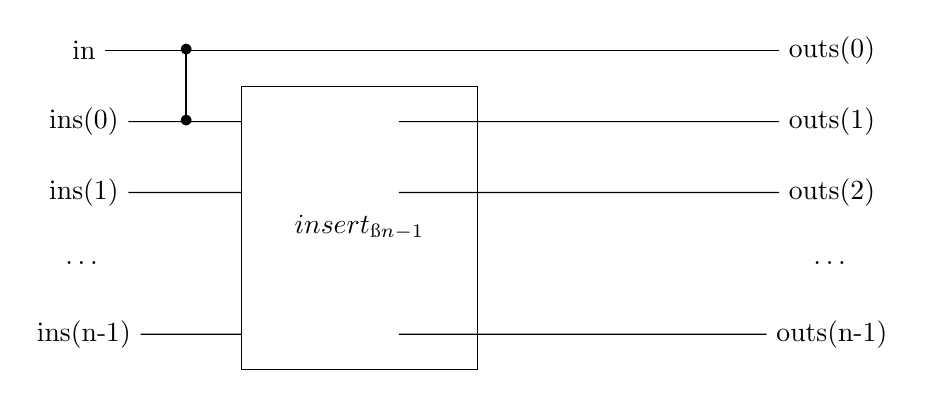
\begin{tikzpicture}[yscale = 0.9]
% First row
\draw(0,0) node (in) {\scalashape in};
\draw(\width,0) node (outs0) {\scalashape outs(0)};
\draw (in)--(outs0);
% Recursive insert box
\draw (\recX+1.5,-2.5) node {$\sm{insert}_{\ss n-1}$};
\draw (\recX,-0.5) -- ++(3,0) -- ++ (0,-4) -- ++(-3,0) -- ++ (0,4);
% Second row
\draw (0,-1) node (ins0) {\scalashape ins(0)};
\draw (ins0) -- (\recX,-1);
\comp{in}{ins0}{1.3};
\draw (\width,-1) node (outs1) {\scalashape outs(1)};
\draw (\recEnd,-1) -- (outs1);
%
\draw (0,-2) node (ins1) {\scalashape ins(1)};
\draw (ins1) -- (\recX,-2);
\draw (\width,-2) node (outs2) {\scalashape outs(2)};
\draw (\recEnd,-2) -- (outs2);
%
\draw (0,-3) node {\ldots};
\draw (\width,-3) node {\ldots};
%
\draw (0,-4) node (inslast) {\scalashape ins(n-1)};
\draw (inslast) -- (\recX,-4);
\draw (\width,-4) node (outslast) {\scalashape outs(n-1)};
\draw (\recEnd,-4) -- (outslast);
\end{tikzpicture}
\end{center}
%
\begin{qpart}
\label{Q:insert1}
Study the circuit and persuade yourself that it indeed implements the
requirements.  Then implement |insert| based upon the circuit.  You will also
need a base case, for $\sm n = 1$.  Test the circuit.
\end{qpart}

%%%%%

%% %\begin{question}
%% \label{Q:insert2}
%% \textbf{Optional:} The circuit from the previous question had a path
%% containing $O(n)$ comparators.  Design, implement and test a circuit for
%% |insert| such that the longest path has length $O(\log n)$.
%% %\end{question}

%%%%%

\begin{qpart}
Use your function from part~\ref{Q:insert1} to implement insertion sort.  Use
the following signature.
%
\begin{scala}
  /** Insertion sort. */
  def insertionSort(ins: List[??[Int]], outs: List[!![Int]]): ThreadGroup = {
    val n = ins.length; require(n >= 2 && outs.length == n)
    ...
  }
\end{scala}
%
You should base your implementation on the following cicuit, where the
sub-circuit $\sm{iSort}_{\ss n-1}$ recursively sorts $\sm n-1$ inputs.

\begin{center}
\def\width{9.5} % x coord for output labels
\def\recStart{1.5} % X coord for start of recursive iSort
\def\recWidth{2.5} % width of recursive iSort
\def\recEnd{\recStart+\recWidth} % X coord of right edge of recursive iSort
\def\insStart{5.5}
\def\insWidth{2.5}
\def\insEnd{\insStart+\insWidth}
%
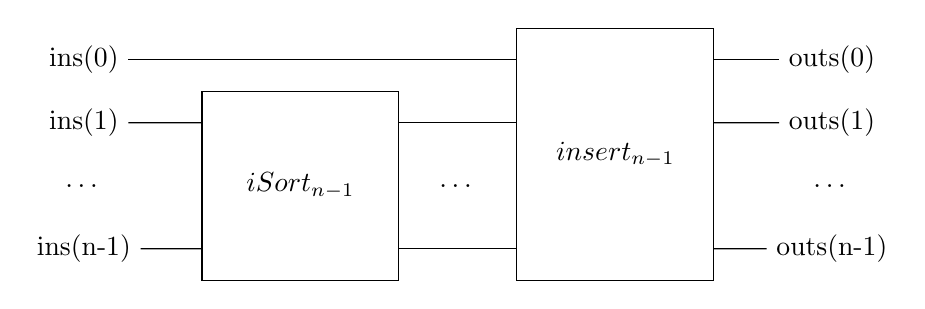
\begin{tikzpicture}[yscale = 0.8]
% Top row
\draw(0,0) node (ins0) {\scalashape ins(0)};
\draw(\width,0) node (outs0) {\scalashape outs(0)};
\draw (ins0)--(\insStart,0); \draw (\insEnd,0)--(outs0);
% Recursive iSort box
\draw (\recStart+1.25,-2.0) node {$\sm{iSort}_{\sm n-1}$};
\draw (\recStart,-0.5) -- ++(\recWidth,0) -- ++(0,-3) -- ++(-\recWidth,0) -- 
  ++(0,3);
% Insert box
\draw (\insStart+1.25,-1.5) node {$\sm{insert}_{\sm n-1}$};
\draw (\insStart,+0.5) -- ++(\insWidth,0) -- ++(0,-4) -- ++(-\insWidth,0) --
  ++(0,4);
% Second row
\draw (0,-1) node (ins1) {\scalashape ins(1)};
\draw (ins1) -- (\recStart,-1);
\draw (\recEnd,-1) -- (\insStart,-1);
\draw (\width,-1) node (outs1) {\scalashape outs(1)};
\draw (\insEnd,-1) -- (outs1);
% Third row
\draw (0,-2) node  {\ldots};
\draw (\recEnd+0.75,-2) node  {\ldots};
\draw(\width,-2) node {\ldots};
% Last row
\draw (0,-3) node (inslast) {\scalashape ins(n-1)};
\draw (inslast) -- (\recStart,-3);
\draw (\recEnd,-3) -- (\insStart,-3);
\draw (\width,-3) node (outslast) {\scalashape outs(n-1)};
\draw (\insEnd,-3) -- (outslast);
\end{tikzpicture}
\end{center}
%
Test your implementation using the ideas from part~\ref{Q:sort4}.
\end{qpart}

%%%%%

%% \subsection*{Just for fun}

%% Finally, we will implement a technique known as \emph{bitonic
%%   sorting}.  The idea is closely based on merge sort: small inputs are
%% sorted directly; larger inputs are split into two; each half is sorted
%% recursively; and the results are merged together.  For simplicity, we
%% will assume that the number of inputs is a power of~2.

%% The merging circuit can be defined recursively.  The base case is
%% straightforward.  Below is the merging circuit for eight inputs, making use of
%% two four-input merge circuits and four comparators.  It assumes that the two
%% halfs of the input, $\seq{x_0,x_1,x_2,x_3}$ and $\seq{x_4,x_5,x_6,x_7}$ are
%% each sorted, and merges them into a single sorted sequence.
%% %
%% \begin{center}
%% \begin{tikzpicture}[scale = 0.4, >=angle 90,shorten >=1pt]
%% % input wires
%% \foreach \y/\i in {4/1,3/2,2/3,1/4,-1/5,-2/6,-3/7,-4/8}
%%   \node (x\i) at (-0.6,\y){$x_{\i}$};
%% \foreach \y/\z in {4/4,3/-1,2/3,1/-2,-1/-3,-2/2,-3/-4,-4/1}
%%   \draw(0,\y) -- (4,\z);
%% % mergers
%% \draw(4,-0.5) rectangle (9,-4.5);
%% \node at (6.5,-2.5) {$Merge(4)$};
%% \draw(4,0.5) rectangle (9,4.5);
%% \node at (6.5,2.5) {$Merge(4)$};
%% % connecting wires
%% \foreach \y/\z in {4/4, 3/2, 2/-1, 1/-3, -1/3, -2/1, -3/-2, -4/-4}
%%   \draw(9,\y) -- (13,\z);
%% % comparators
%% \foreach \y/\z in {4/3, -1/-2, 2/1, -3/-4}{
%%   \draw (13,\y) node {$\bullet$};
%%   \draw (13,\z) node {$\bullet$};
%%   \draw[thick] (13,\y) -- (13,\z);
%% }
%% %\foreach \y in {3.5,1.5,-1.5,-3.5}
%%   % \draw(13,\y-0.8) rectangle (14,\y+0.8);
%% %outputs
%% \foreach \y in {4,3,2,1,-1,-2,-3,-4}
%%   \draw(13,\y) -- (15,\y);
%% \foreach \y/\i in {4/1,3/2,2/3,1/4,-1/5,-2/6,-3/7,-4/8}
%%   \node at (15.5,\y){$y_{\i}$};
%% \end{tikzpicture}
%% \end{center}
%% %
%% Each half of the input is split between the two sub-merges.  Corresponding
%% outputs from the two sub-merges are fed into comparators.

%% %\begin{question}
%% Implement this sorting algorithm.  Use the following signature, for a circuit
%% for $2^k$ values.
%% %
%% \begin{scala}
%%   /** A merging network for £$2^k$£ values.  If the values received on
%%     * ins1 and ins2 are sorted, then their merger is output on outs. */
%%   def merge(k: Int)(ins1: List[?[Int]], ins2: List[?[Int]], outs: List[![Int]])
%%       : ThreadGroup = {
%%     val n = 1 << k; val halfN = n/2
%%     require(k >= 1 && ins1.length == halfN && ins2.length == halfN &&
%%               outs.length == n)
%%     ...
%%   }
%% \end{scala}
%% %
%% You might want to use the following function for doing the splitting.
%% \begin{scala}
%%   /** Split xs into two lists, alternately.
%%     * @return the lists <xs(0), xs(2), xs(4),...> and <xs(1), xs(3), xs(5), ...>
%%     */
%%   private def split[T](xs: List[T]): (List[T], List[T]) = 
%%     if(xs.isEmpty) (List[T](), List[T]())
%%     else{ val (ys, zs) = split(xs.tail); (xs.head::zs, ys) }
%% \end{scala}
%% %\end{question}

%% %%%%%

%% The sorting circuit itself can also be defined recursively.  The base case is
%% straightforward.  The recursive case is illustrated below: the input is split
%% in half; each half is sorted; the results are merged.
%% % 
%% \begin{center}
%% \begin{tikzpicture}[scale = 0.4, >=angle 90,shorten >=1pt]
%% \foreach \y in {4,3,2,1,-1,-2,-3,-4}
%%   \draw(0,\y) -- (1,\y);
%% \draw(1,0.5) rectangle (6,4.5);
%% \node at (3.5,2.5) {$sort(n)$};
%% \draw(1,-0.5) rectangle (6,-4.5);
%% \node at (3.5,-2.5) {$sort(n)$};
%% \foreach \y in {4,3,2,1,-1,-2,-3,-4}
%%   \draw(6,\y) -- (8,\y);
%% \draw(8,-4.5) rectangle (14,4.5);
%% \node at (11,0){$merge(2n)$};
%% \foreach \y in {4,3,2,1,0,-1,-2,-3,}
%%   \draw(14,\y-0.5) -- (15,\y-0.5);
%% \end{tikzpicture}
%% \end{center}

%% %\begin{question}
%% Implement this sorting circuit.  Use the following signature.
%% %% \footnote{You
%%   %% might want to use the operations {\scalashape take} and {\scalashape drop}
%%   %% from the {\scalashape List} class for splitting the input.}
%% %
%% \begin{scala}
%%   /** A bitonic sorting network for 2^k values. */
%%   def bitonicSort(k: Int)(ins: List[?[Int]], outs: List[![Int]]): ThreadGroup = {
%%     val n = 1 << k
%%     require(ins.length == n && outs.length == n)
%%     ...
%%   }
%% \end{scala}

%% Test your implementation using the ideas from Question~\ref{Q:sort4}.
%\end{question}
\end{question}

%%%%%%%%%%%%%%%%%%%%%%%%%%%%%%%%%%%%%%%%%%%%%%%%%%%%%%%

\begin{answerI}
Most of the code consists of fairly straightforward translations of the
diagrams. 
%
\begin{enumerate}
\item
%\begin{qpart}
\begin{scala}
  def comparator(in0: ??[Int], in1: ??[Int], out0: !![Int], out1: !![Int])
    = thread("comparator"){
    var x0 = -1; var x1 = -1
    repeat{
      run(thread{ x0 = in0?() } || thread{ x1 = in1?() })
      run(thread{ out0!(x0 min x1) } || thread{ out1!(x0 max x1) })
    }
    in0.close(); in1.close(); out0.endOfStream(); out1.endOfStream()
  }
\end{scala}
%\end{qpart}

%%%%%

\item
%\begin{qpart}
\begin{scala}
  def sort4(ins: List[??[Int]], outs: List[!![Int]]): ThreadGroup = {
    require(ins.length == 4 && outs.length == 4)
    val c0, c1, c2, c3, c4, c5 = new SyncChan[Int]
    comparator(ins(0), ins(2), c0, c2) ||
      comparator(ins(1), ins(3), c1, c3) ||
      comparator(c0, c1, outs(0), c4) ||
      comparator(c2, c3, c5, outs(3)) ||
      comparator(c4, c5, outs(1), outs(2))
  }
\end{scala}
%\end{qpart}

\item
\begin{scala}
  def insert(ins: List[??[Int]], in: ??[Int], outs: List[!![Int]])
      : ThreadGroup = {
    val n = ins.length; require(n >= 1 && outs.length == n+1)
    if(n == 1) comparator(ins(0), in, outs(0), outs(1))
    else{
      val c = new SyncChan[Int]
      comparator(in, ins(0), outs(0), c) || insert(ins.tail, c, outs.tail)
    }
  }
\end{scala}


\item
\begin{scala}
  def insertionSort(ins: List[??[Int]], outs: List[!![Int]]): ThreadGroup = {
    val n = ins.length; require(n >= 2 && outs.length == n)
    if(n == 2) comparator(ins(0), ins(1), outs(0), outs(1))
    else{
      val mids = List.fill(n-1)(new SyncChan[Int])
      insertionSort(ins.tail, mids) || insert(mids, ins(0), outs))
    }
  }
\end{scala}
\end{enumerate}
\end{answerI}
 % sorting using comparators


% More exercises: Bitonic part of sorting practical?
